\subsection*{Problema 25}

\textbf{Enunciado:} Calcular la integral trigonométrica:
\begin{align*}
I = \int \dfrac{dx}{4\sin^2 x + 9\cos^2 x}
\end{align*}

\textbf{Solución:} Siguiendo las indicaciones, dividimos tanto el numerador como el denominador por $\cos^2 x$:
\begin{align*}
I &= \int \dfrac{\dfrac{1}{\cos^2 x}}{\dfrac{4\sin^2 x}{\cos^2 x} + \dfrac{9\cos^2 x}{\cos^2 x}} dx \\
I &= \int \dfrac{\sec^2 x}{4\tan^2 x + 9} dx
\end{align*}

Realizamos la sustitución sugerida. Sea $u = \tan x$, entonces su derivada es:
\begin{align*}
du = \sec^2 x \, dx
\end{align*}

Sustituyendo $u$ y $du$ en la integral, obtenemos una forma estándar de integración:
\begin{align*}
I &= \int \dfrac{du}{4u^2 + 9} \\
I &= \int \dfrac{du}{(2u)^2 + 3^2}
\end{align*}

Aplicamos la fórmula de integración $\int \dfrac{dw}{w^2 + a^2} = \dfrac{1}{a}\arctan\left(\dfrac{w}{a}\right) + C$, donde $w = 2u$, $dw = 2 du$ y $a = 3$:
\begin{align*}
I &= \dfrac{1}{2} \int \dfrac{2 \, du}{(2u)^2 + 3^2} \\
I &= \dfrac{1}{2} \cdot \dfrac{1}{3} \arctan\left(\dfrac{2u}{3}\right) + C \\
I &= \dfrac{1}{6} \arctan\left(\dfrac{2u}{3}\right) + C
\end{align*}

Finalmente, regresamos a la variable original $x$ sustituyendo $u = \tan x$:
\begin{align*}
I = \dfrac{1}{6} \arctan\left(\dfrac{2\tan x}{3}\right) + C
\end{align*}

\begin{figure}[H]
	\centering
	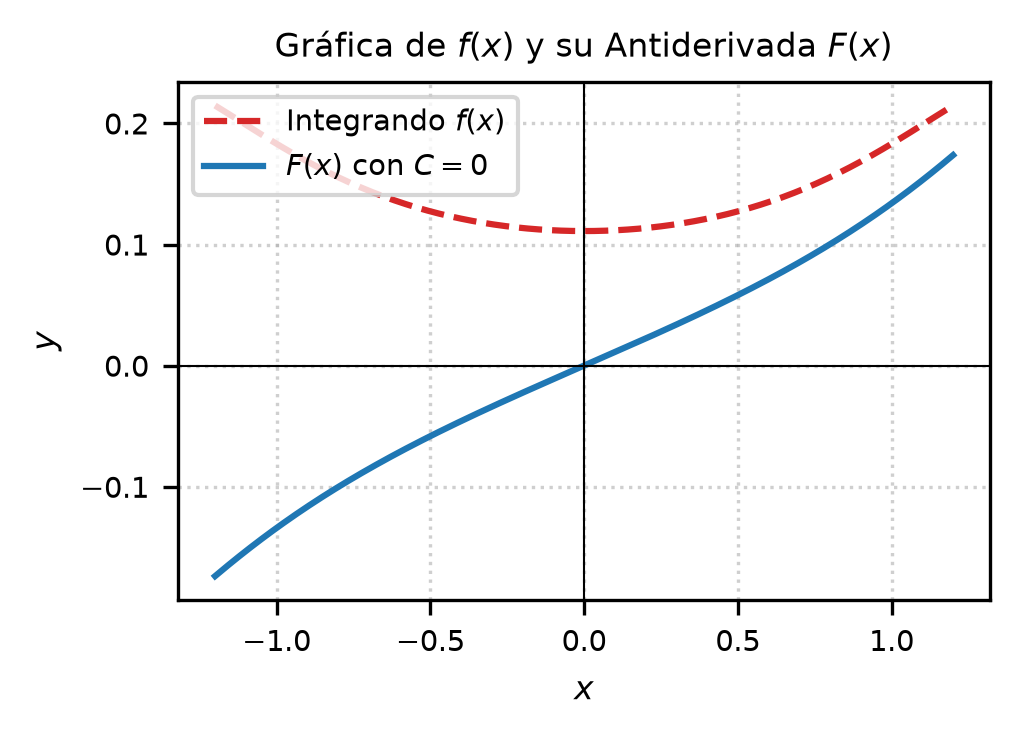
\includegraphics[width=\columnwidth]{semana_04/graficas/SEM04_P25_grafica.png}
	\caption{Representación gráfica de $f(x)$ y su antiderivada $F(x)$ evaluada para la constante de integración $C = 0$ (Problema 25).}
	\label{fig:problema25}
\end{figure}
